\section{THEORETICAL ANALYSIS}
\label{sec:proof}

This section proves that CS-G-FR and CS-G-OMP 
produce near-optimal explained variance $F$ at budgets 
where features are selected. The main challenge of our analysis is to prove Lemma~\ref{lemma:main},
%which relates the marginal performance gain at step $j$,
%$F(G_j) - F(G_{j-1})$, to 
%the performance difference, $F(S) - F(G_{j-1})$, between 
%a competing sequence $S$ and the current greedy sequence $G_{j-1}$. 
which is a common stepping stone in 
submodular maximization analysis, e.g., Equation 8 in \citep{submodular}. The main Theorem~\ref{thm:main} follows from the lemma by standard techniques, which we defer to the appendix. 

\begin{lemma}[main]
  Let $G_j$ be the first $j$ feature groups selected by our greedy algorithm. There exists a constant $\gamma = \frac{\lambda^* + \lambda}{1 +\lambda} > 0$ such that for any sequence $S$, total cost $K$, and indices $j=1,2,..., J$, 
  \mbox{$
    F(S_{\angleb{K}}) - F(G_{j-1}) \leq \frac{K}{\gamma}
      \lbrack \frac{F(G_j) - F(G_{j-1})}{c(g_j)} \rbrack.
  $}
  \label{lemma:main}
\end{lemma}


\begin{theorem}
Let $B = \sum _{i=1}^L c(g_i)$ for some $L$.  
There exists a constant  
  $\gamma = \frac{\lambda^* + \lambda}{1+\lambda}$, 
  such that
for any sequence $S$ and total cost $K$, 
\mbox{$
  F(G_{\angleb{B}}) > (1 - e^{-\gamma\frac{B}{K}})F(S_{\angleb{K}}).
$}
\label{thm:main}
\end{theorem}

%
% Theorem implication 
Before delving into the proof of Lemma~\ref{lemma:main}, we first discuss 
some implications of Theorem~\ref{thm:main}, which 
argues that the explained variance of greedily selected
features of cost $B$ is within $(1-e^{\gamma \frac{B}{K}})$-factor
of that of any competing feature sequence of cost $K$.
If we apply minimum regularization $(\lambda \rightarrow 0)$, then 
the constant $\gamma$ approaches $\lambda^*$. The resulting bound factor $(1-e^{ - \lambda^* \frac{B}{K}})$ is the bound for FR by \cite{kemp}. However, we achieve the same bound for OMP, improving
theoretical guarantees of OMP. We also note that less-correlated features lead
to a higher $\lambda^*$  and a stronger bound. 


%If all feature groups are uncorrelated, then $C = (1 + \lambda)I$ so that $\gamma = 1$. If features have linear dependencies, then 
%$\gamma = \frac{\lambda}{1+\lambda}$, since $\lambda_{min}(C) = \frac{1}{n} \lambda_{min}(X^TX) + \lambda = \lambda$, where $X^TX$ is a singular matrix. In this case, the bound solely depends on regularization $\lambda$. In general, however, the less feature groups are correlated, the higher is $\lambda_{min}(C)$, and the better is the bound. 



% CS-G-FR. claim for CS-G-OMP
Lemma~\ref{lemma:main} for CS-G-FR is standard if we follow proofs in \citep{streeter:08} and \citep{kemp} because the objective $F$ is $\gamma$-approximately submodular. 
%$\gamma$ is then proven in \cite{kemp} to no smaller than $\lambda^*$. 
However, we present a proof of 
Lemma~\ref{lemma:main} for CS-G-OMP without approximate submodularity to achieve the same constant $\gamma$. 
This proof in turn uses Lemma~\ref{lemma:smoothness} and Lemma~\ref{lemma:convexity}, whose proofs are based on the Taylor expansions of the regularized risk $\mathcal{R}[f_S]=R(S)$, a $M$-strongly smooth and $m$-strongly convex loss functional of predictors $f(x) = w^T x$.
We defer these two proofs to the appendix and note that 
$M=m$ with our choice of $R$. 



%%%%%%%%%%%%%
%%%%%%  Theorem.
%Let $G = g_1, g_2, ... , g_{J}$ be the sequence of feature groups that our CS-G-OMP selects. Let $S$ be any sequence of feature groups. For any $B$ such that $B = \sum _{j=1}^{L} c(g_j)$ for some $L$, let $G_{\angleb{B}}$ be the first $L$ feature groups of $G$, $g_1, g_2, ..., g_{L}$. We denote $S_{\angleb{K}} = s_1, s_2, ... $ to be any competing sequences of cost $K$, that is, $\sum _{j=1.. J : \mathcal{G}_j \subseteq S_{\angleb{K}}} c(\mathcal{G}_j) = K$. For any two selected feature group sequence $G$ and $S$, we define $b^G_S$ as the gradient of the objective $F(G)$ with respect to coefficient of  group $S$, $w_S$; components of $b^G_S$ can be computed using $b^G_g$ defined in Equation~\ref{eq:bG}.  We define matrix $C$ to be $C \triangleq \frac{1}{n}X^TX + \lambda I$, which is the regularized covariance matrix of features. Let the minimum eigenvalue of $C$ be $\lambda _{min}(C) = \frac{1}{n}\lambda_{min}(X^TX) + \lambda > 0$.

%Then our main results below bounds $F(G_{\angleb{B}})$, the explained variance achieved using proposed features, with a constant factor of $F(S_{\angleb{K}})$, 
%the explained variance of any competing sequence with budget $K$. 


 
%The proof of the theorem relies on Lemma~\ref{lemma:main}, which mimics a classical result in submodular maximization literature such as Equation 8 of \cite{submodular}. From Lemma~\ref{lemma:main}, the proof is a standard technique in approximate submodular maximization literature, which we defer to the appendix. 

%%%%%%%%%%%%%
%%%%%%%% Lemma approximately submodularity
%\begin{lemma}[main]
%  There exists constant $\gamma = \frac{\lambda _{min}(C)}{1+\lambda} > 0$ such that for all $S$ and total cost $K$,  and all $j=1,2,..., J$, 
%  \mbox{$
%    F(S_{\angleb{K}}) - F(G_{j-1}) \leq \frac{K}{\gamma}
%      \lbrack \frac{F(G_j) - F(G_{j-1})}{c(g_j)} \rbrack.
%  $}
%  \label{lemma:main}
%\end{lemma}

%%%%%%%%%%%%% 
%%%%%%%   Lemma Strong smoothness
\begin{lemma}[Using Smoothness]
  Let $S$ and $G$ be some fixed sequences. Then
  \mbox{$
    F(S) - F(G) \leq \frac{1}{2m} \angleb{b^G_{G \oplus S}, C_{G \oplus S}^{-1} b^G_{G\oplus S}}.
  $}
  \label{lemma:smoothness}
\end{lemma}

%%%%%%%%%%%%% 
%%%%%  Lemma Strong convexity
\begin{lemma}[Using Convexity] For $j = 1,2,..., J$, 
    \mbox{$
      F(G_j) - F(G_{j-1}) \geq \frac{1}{2M} \angleb{ {b^{G_{j-1}}_{g_j}}, C_{g_j}^{-1}b^{G_{j-1}}_{g_j} }.
    $}
  \label{lemma:convexity}
\end{lemma}
Note that in Lemma~\ref{lemma:convexity}, since we assume feature groups are 
whitened, then $C_{g_j} = (1+\lambda) I$. The bound of the lemma becomes
$F(G_j) - F(G_{j-1}) \geq \frac{1}{2M (1+\lambda)} \angleb{ {b^{G_{j-1}}_{g_j}}, b^{G_{j-1}}_{g_j} }$. If feature groups are not whitened, 
the constant $(1+\lambda)$ can be scaled up to $(|\mathcal{G}_j| + \lambda)$, 
which detriments the strength of Theorem~\ref{thm:main} especially when feature 
groups are large. 


\begin{proof} (of Lemma~\ref{lemma:main}, using Lemma~\ref{lemma:smoothness} and Lemma~\ref{lemma:convexity}) \\
  Using Lemma ~\ref{lemma:smoothness}, on $S_{\angleb{K}}$ and $G_{j-1}$, we have: 
  \begin{align}
    &F(S_{\angleb{K}}) - F(G_{j-1})  \notag \\
    &\leq 
      \frac{1}{2m} \angleb{b^{G_{j-1}}_{G_{j-1} \oplus S_{\angleb{K}}},
      C^G_{G_{j-1} \oplus S_{\angleb{K}}} b^{G_{j-1}}_{G_{j-1} \oplus S_{\angleb{K}}}}
  \end{align}
  Note that the gradient $b_{G_{j-1}}^{G_{j-1}}$  
  		equals $0$, because $F(G_{j-1})$ is achieved by  
  		the linear model $w(G_{j-1})$. Then, using block matrix inverse
  formula, we have:
  \begin{align}
    F(S_{\angleb{K}}) - F(G_{j-1}) \leq 
      \frac{1}{2m} 
      \angleb{b^{G_{j-1}}_{S_{\angleb{K}}},
      C^G_{S_{\angleb{K}}} 
      b^{G_{j-1}}_{S_{\angleb{K}}}}
  \end{align}
  where $
    C^G_{S_{\angleb{K}}} = C_{S_{\angleb{K}}} - C_{{S_{\angleb{K}}}G} 
      C^{-1}_{S_{\angleb{K}}} C_{G{S_{\angleb{K}}}}.  $
  Using spectral techniques in Lemmas 2.5 and 2.6 in \citep{kemp} and
  noting that the minimum eigenvalue of $C$, $\lambda_{min}(C)$, is $\lambda^* + \lambda$, we have
  \begin{align}
      \frac{1}{2m} 
      \angleb{b^{G_{j-1}}_{S_{\angleb{K}}}, 
      C^G_{S_{\angleb{K}}} 
      b^{G_{j-1}}_{S_{\angleb{K}}}}
    \leq 
      \frac{1}{2m (\lambda^* + \lambda)} 
     \angleb{b^{G_{j-1}}_{S_{\angleb{K}}}, 
      b^{G_{j-1}}_{S_{\angleb{K}}}}.
  \end{align}
  Expanding $S_{\angleb{K}}$ into individual groups $s_i$, we continue:
  \begin{align}
    &= 
    	\frac{1}{2m(\lambda^* + \lambda)} \sum _{s_i \in S_{\angleb{K}}} 
       \angleb{b^{G_{j-1}}_{s_i}, {b^{G_{j-1}}_{s_i}}}  \\
    &\leq
        \frac{1}{2m(\lambda^* + \lambda)} \sum _{s_i \in S_{\angleb{K}}} 
        c(s_i) \max_{g} \frac{  \angleb{b^{G_{j-1}}_{g}, {b^{G_{j-1}}_{g}}}}{c(g)} \\
    &=
        \frac{1}{2m(\lambda^* + \lambda)} \sum _{s_i \in S_{\angleb{K}}} 
        c(s_i) \frac{\angleb{b^{G_{j-1}}_{g_j}, {b^{G_{j-1}}_{g_j}}}}{c(g_j)} \\
    &\leq
        \frac{ M(1+ \lambda)}{m (\lambda^* + \lambda)} \sum _{s_i \in S_{\angleb{K}}} 
        c(s_i)
          \frac{ F(G_{j}) - F(G_{j-1}) } { c(g_j) }.
  \end{align}
  The last equality follows from the greedy selection step of Algorithm~\ref{algo:gomp_lm} when feature groups are whitened. 
  The last inequality is given by Lemma ~\ref{lemma:convexity}. The 
  theorem then follows from $\gamma = (\frac{m}{M}) \frac{\lambda^* + \lambda}{1+\lambda} = \frac{\lambda^* + \lambda}{1+\lambda}$. 
\end{proof}




        
        


\section{BI-CRITERIA APPROXIMATION AT ALL BUDGETS}

Our analysis so far only bounds algorithm performance at 
budgets when new items are selected. However, an ideal analysis
should apply to all budgets. As illustrated in Figure~\ref{fig:all-budget-bad},
previous methods may choose expensive features early; 
until they are computed, we have no bounds. 
Figure~\ref{fig:all-budget-good} illustrates our proposed fix: each 
new item $g_{j+1}$ cannot be more costly than the current sequence $G_{j}$. 

This section proves two theorems of anytime prediction at \textit{any} budget.  Theorem~\ref{thm:greedy.biapproximation-upper-bound} shows that
 to approximate the optimal explained variance 
of cost $B$ within a constant factor,
an anytime algorithm must cost at least $4B$. 
We then motivate and formalize our fix in Algorithm~\ref{alg:greedy.doubling},
which is shown in
Theorem~\ref{thm:greedy.doubling-greedy-bound-approx} to achieve this
\textit{bi-criteria approximation} bound for both budget and objective with
the form: \mbox{$F(G_{\at{B}}) > (1 - e^{-\frac{\gamma^2}{1+\gamma}}) F(S_{\at{\frac{B}{4}}})$}, where $\gamma$ is the approximate submodular
ratio, i.e., the maximum constant $\gamma \leq 1$ such that for 
all sets $ A' \subseteq A$ and all element $x$,
\begin{equation}
\label{def:greedy.approx-submodularity}
    \gamma (F(A \cup \{x\}) - F(A)) \leq F(A' \cup \{x\}) - F(A').
\end{equation}
%in \cite{kemp} and satisfies the following for all 
%set $A$ and $S$,
%\begin{equation}
%\label{def:greedy.approx-submodularity}
%\gamma \left[F(A \cup S) - F(A)\right]
%  \le \sum_{x \in S} \left[F(A \cup \{x\}) - F(A)\right].
%\end{equation}
%Noting the positively-weighted average of non-negative elements 
%is no greater than the maximum element, 
%we have:
%$
%\label{def:greedy.approx-submodularity-rate}
%\gamma \left[\frac{F(A \cup S) - F(A)}{c(S)} \right] 
%\leq \max _{x\in S} \frac{F(A \cup \{x\}) - F(A)}{c(x)}.
%$
%To our knowledge, Theorem~\ref{thm:greedy.biapproximation-upper-bound} and~\ref{thm:greedy.doubling-greedy-bound-approx} are 
%the first anytime algorithm analyses at \textit{all} budgets instead
%of at specific budgets (such as when features are chosen).

We first illustrate the inherent difficulty in 
generating single sequences that are competitive at arbitrary budgets
$B$ by using the following budgeted maximization problem:
\begin{align}
\label{eq:greedy.hard-problem}
X = \{1,2,\ldots\},\;\; c(x) = x, \;\;
F(S) = \sum_{x \in S} e^x.
\end{align}
The above problem originates from fitting the linear model
$Y = \sum _{i=1}^D e^iX_i$, where $X_i$'s are i.i.d. and $X_i$ 
costs $i$. 

\begin{theorem}
\label{thm:greedy.biapproximation-upper-bound}
Let $\mathcal{A}$ be any algorithm for selecting sequences $A = (a_1,
\ldots)$.  The best bi-criteria approximation that $\mathcal{A}$ can
satisfy must be at least a $4$-approximation in cost for the sequence
described in Equation~(\ref{eq:greedy.hard-problem}).  That is, there
does not exist a $C < 4$, and a $c_1 \in [0,1)$, such that for any budget $B$ and
any sequence $S$,
\[
F(A_{\at{B}}) > \left(1 - c_1\right) F(S_{\at{\frac{B}{C}}}).
\]
\end{theorem}

\begin{proof}
For any budget $B$, it is clear that the optimal selection contains
a single item, $B$, whose value is $e^B$. 
For any budget $B$, let $m(B)$ denote the item of the maximum cost that is selected by the algorithm.
If the bi-criteria bound holds, then 
$\sum _{k=1}^{m(B)} e^k \geq F(A_{\at{B}}) > \left(1 - c_1\right) F(S_{\at{\frac{B}{C}}})$. 
Taking the log of both sides and rearranging terms, we have $m(B) \geq \lfloor \frac{B}{C} \rfloor + \ln(1-c_1) + \ln(e-1) - 2$. 
Since $3 - \ln (1-c_1) - \ln (e-1) > 0$,  we have for $B$ large enough:
$C \geq \frac{B}{m(B)}. $ 
Hence, we need to minimize $\frac{B}{m(B)}$ for all $B$ to minimize $C$. We
can assume $a_j$ to be increasing 
because otherwise we could remove the violating $a_j$ 
from the sequence and decrease the ratio $\frac{B}{m(B)}$ for all subsequent $j$. 

Let $b_j := c(A_j)$ and $\alpha_{j} := \frac{c(a_{j})}{b_{j-1}}$. 
Then immediately before $a_{j}$ is available,
$\frac{B}{m(B)} \rightarrow 
\frac{c(A_j)}{c(a_{j-1})} \geq \frac{(1+\alpha_j)b_{j-1}}{b_{j-1}} = 1+\alpha_j$. If we can bound $\frac{B}{m(B)}\leq C$ for all $B$, 
then there exists $\alpha_{max}$ such that
$\alpha_j < \alpha_{max}$ for all $j$ large enough. 
Immediately after a new $a_j$ is selected, 
$\frac{B}{m(B)} = \frac{c(A_j)}{c(a_{j})} = \frac{1+\alpha_j}{\alpha_j}$. 
For $\frac{B}{m(B)}$ to be bounded, there must exist some $\alpha_{min}>0$ such that
$\alpha_j > \alpha_{min}$ for large enough $j$.
Now we consider the ratio $\frac{B}{m(B)}$ right before $a_{j+1}$ is selected:
\begin{align}
\hspace{-13pt} \frac{c(A_{j+1})}{c(a_{j})}= \frac{b_j(1+\alpha_{j+1})}{b_j\frac{\alpha_{j}}{1+\alpha_j}} =  
1 + \frac{\alpha_{j+1}}{\alpha_j} + \alpha_{j+1} + \frac{1}{\alpha_j}.
\label{line:lower_bound_cost_ratio}
\end{align}
Assume for seek of contradiction that $\frac{c(A_{j+1})}{c(a_{j})}$ 
is bounded above by $z$ for some $z \in (1,  4)$.
Let $y := \frac{\alpha_{j+1}}{\alpha_j}$. Then we have:
$ z \geq 1 + y + y\alpha_j + \frac{1}{\alpha_j} \geq 1 + y + 2\sqrt{y} = (\sqrt{y} + 1)^2$. Hence $y \leq (\sqrt{z} -1)^2 < 1$. 
So \mbox{$a_{j+1} \leq (\sqrt{z} -1)^2 a_j$}, which implies that $a_j$ converges to $0$ and we have a contradiction.
So \mbox{$C \geq \frac{B}{m(B)}  \rightarrow \frac{c(A_{j+1})}{c(a_{j})} \geq 4$} for large $j$.
\end{proof}

The above proof lower bounds the cost approximation ratio $C$ by Eq.~\ref{line:lower_bound_cost_ratio}, which is shown to be at least $4$ for $C < \infty$. We note that $Eq.~\ref{line:lower_bound_cost_ratio}$ equals $4$ if $\forall j, \alpha_j = 1$, which means the sequence total cost is doubled at each selection step.
This observation leads to \textit{Doubling Algorithm} (Alg.~\ref{alg:greedy.doubling}): we perform greedy selection in the same way as CS-G-FR, except that the total cost can be at most doubled at each step (illustrated in Figure~\ref{fig:doubling-algo}). 
The advantage of Doubling Algorithm over 
CS-G-FR is that 
the former prevents early computation of expensive features and induces a smoother increase of total cost; in most real-world data-sets, the two are identical after few steps because 
feature costs are often in a narrow range. 
We will analyze Doubling Algorithm with the following assumption, called \textit{doubling capable}.

\begin{figure}
\centering
\subfloat[Before $F$ is computed, we have no output or bounds.]{
  
\includegraphics[width=0.49\textwidth]{\GOMPDIR/img/all-budget-bad.png}
  \label{fig:all-budget-bad}
}

\subfloat[Our constraint $c(g_{j+1}) \leq c(G_j)$ induces a smoother cost increase. ] {
  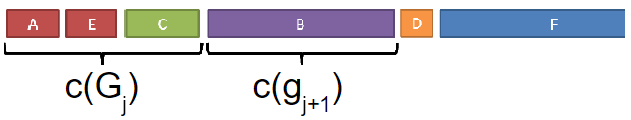
\includegraphics[width=0.49\textwidth]{\GOMPDIR/img/all-budget-good.png}
  \label{fig:all-budget-good}
}

\subfloat[Illustration of Doubling Algorithm Cost Constraint]{
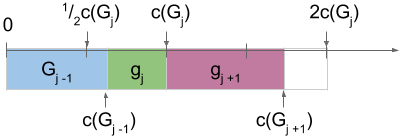
\includegraphics[width=0.45\textwidth]{\GOMPDIR/img/doubling-algo.png}
  \label{fig:doubling-algo}
}

\caption{Doubling Algorithm (b) has better anytime behaviors 
than greedy algorithm with no cost constraints (a).}
\label{fig:doubling}
\end{figure}


%\begin{algorithm}[t]
%  \caption{Doubling Algorithm}
%  \label{alg:greedy.doubling}
%  
%  \SetKwInOut{Input}{input}
%    \Input{ objective function $F$, elements $X$, minimum cost $c_{\textrm{min}}$}
%    
%    Let $g_1 = \underset{x \in X,\ c(x) \le c_{\textrm{min}}}{\argmax} \frac{F(\{x\})}{c(x)}$; 
%    Let $G_1 = g_1$ \;
%    \For{$j = 2,\ldots$} {
%    Let $g_j = \underset{x \in X \setminus G_{j-1},\ c(x) \le c(G_{j-1})}{\argmax} \;
%      \frac{F(G_{j-1} \oplus \{x\}) - F(G_{j-1})}{c(x)}$ \;
%    Let $G_j = G_{j-1} \oplus \{g_j\}$ \;
%    }
%\end{algorithm}

 
\begin{definition} 
\label{def:greedy.doubling-capable}
Let $G = (g_1, \ldots)$ be the sequence selected by the doubling
algorithm.  The set $X$ and function $F$ are \textit{doubling capable}
if, at every iteration $j$, the following set is non-empty:
$
\{x \mid x \in X \setminus G_{j-1},\ c(x) \le c(G_{j-1})\}
$
\end{definition}

\begin{theorem}
\label{thm:greedy.doubling-greedy-bound-approx}
Let $G = (g_1, \ldots)$ be the sequence selected by the doubling
algorithm (Algorithm~\ref{alg:greedy.doubling}).  Fix some $B >
c_{\textrm{min}}$.  Let $F$ be $\gamma$-approximately
submodular as in Definition~\ref{def:greedy.approx-submodularity}.
For any sequence $S$,
\[
F(G_{\at{B}}) > \left(1 - e^{-\frac{\gamma^2}{1+\gamma}} \right) F(S_{\at{\frac{B}{4}}}).
\]
\end{theorem}
\begin{proof}
Doubling capable easily leads to the observation that for all budgets $B$, there exists an index $j$ such that
$\frac{B}{2} \leq c(G_j) < B$.
Choose $K$ and $k$ to be  the largest integers such that
$\frac{B}{2} \leq c(G_K) < B$ and 
$\frac{B}{8} \leq c(G_k) < \frac{B}{4}$. Since at each step we at most double the 
total cost and $4c(G_k) < B$, we observe $K \geq k+2$. 
%Let $\Delta C$ denote the cost difference $c(G_K) - c(G_k)$.
For each $j$, define $s_j = \frac{F(G_{j+1}) - F(G_{j})}{c(g_{j+1})}$ as the best 
rate of improvement among the items Doubling Algorithm is allowed to consider
after choosing $G_j$. 
Consider the item $x$ in sequence $S_{\at{\frac{B}{4}}}$ of the maximum cost. 

(Case 1) If $c(x) \leq c(G_k)$, then
every item in $S_{\at{\frac{B}{4}}}$ was a candidate for $g_{j}$ for all $j=k+1,..., K$. 
So by approximate submodularity from Equation~\ref{def:greedy.approx-submodularity}, we have 
\begin{align}
\label{eq:sub-additive}
F(S_{\at{\frac{B}{4}}}) \leq F(S_{\at{\frac{B}{4}}} \cup G_{j}) \leq F(G_j) + \frac{B s_j}{4 \gamma}.
\end{align}
Then using the standard submodular maximization proof technique, we define
\mbox{$\Delta _j = F(S_{\at{\frac{B}{4}}}) - F(G_j)$}. Applying $s_j = \frac{\Delta _{j} - \Delta_{j+1}}{c(g_{j+1})}$ in the above inequality, 
we have
\mbox{$\Delta _{k+j} \leq \Delta_k \prod _{j=k+1}^{k+j} ( 1 - \gamma \frac{ 4 c(g_{j})}{B})$}. Maximizing the 
inequality by setting $c(g_{j}) = \frac{B}{K-k} \leq \frac{c(G_K) - c(G_k)}{4 (K-k)}$, 
and using $(1- z/l)^l < e^{-z}$, we have 
\mbox{$F(G_K) > (1 - e^{-\gamma}) F(S_{\at{\frac{B}{4}}}).
$}

From now on, we assume that $c(x) > c(G_k)$ and consider 
two cases by comparing $c(g_{k+2})$ and $c(G_{k})$. 

(Case 2.1) If $c(g_{k+2}) \geq c(G_{k})$, then 
$c(G_K) - c(G_{k+1}) \geq c(g_{k+2}) \geq c(G_k)$. 
Since $c(G_{k+1}) \leq 2 c(G_k)$ and $c(x) > c(G_k)$, 
we have $c(G_K) - c(G_{k+1}) \geq \frac{B}{2} - 2c(G_k)$.
So \mbox{$c(G_K) - c(G_{k+1}) \geq \max ( c(G_k), \frac{B}{2} - 2c(G_k) ) \geq \frac{B}{6}$}. 
Thus, using the same proof techniques as in case 1, we can analyze the ratio between $\Delta_{k+1}$ and $\Delta_K$, and have:
\mbox{$
F(G_K) > (1 - e^{-\frac{2}{3} \gamma}) F(S_{\at{\frac{B}{4}}}).
$}

(Case 2.2) 
Finally, if \mbox{$c(g_{k+2}) < c(G_k) < c(x) < c(G_{k+1})$},
$g_{k+2}$ was a candidate for $g_{k+1}$, and $x$ was a candidate for 
$g_{k+2}$. 
For an item $y$, let 
\mbox{$r(y^j)= \frac{F(G_{j} \cup \{ y \}) - F(G_j)}{c(y)}$} 
be the improvement rate of item $y$ at $G_j$. 
Then we have \mbox{$r(g_{k+1}^k) > r(g_{k+2}^k)$} and \mbox{$r(g_{k+2}^{k+1}) > r(x^{k+1})$}. 
Since the objective function is increasing, we have 
\mbox{$r(x^k) c(x) \leq r(x^{k+1})c(x) + r(g_{k+1}^k)c(g_{k+1})$},
so that 
\mbox{$r(x^k) \leq r(x^{k+1}) + r(g_{k+1}^k) \frac{c(g_{k+1})}{c(x)}$}.
Then by the definition of $\gamma$ in Equation~\ref{def:greedy.approx-submodularity}, we have 
$ \gamma r(g^{k+1}_{k+2}) \leq r(g_{k+2}^k)$. Hence we have 
$ \gamma r(x^{k+1}) \leq  r(g_{k+1}^k)$, which leads to 
\mbox{$r (x^k) \leq r(g_{k+1}^k) (\frac{1}{\gamma} + \frac{c(g_{k+1})}{c(x)} ) \leq r(g_{k+1}^k) (1 + \frac{1}{\gamma})$}. Then
inequality~(\ref{eq:sub-additive}) holds with a coefficient adjustment and becomes
$
F(S_{\at{\frac{B}{4}}}) \leq F(G_k) + \frac{B s_k (1+\gamma)}{4 \gamma^2}.
$
Noting that the above inequality holds for all $j=k+1, ..., K$, we can replace the constant $\gamma$ in the 
proof of case $1$ with $\frac{\gamma^2}{1+\gamma}$ and have the following bound:\mbox{
$
F(G_K) > (1 - e^{-\frac{\gamma^2}{1+\gamma} }) F(S_{\at{\frac{B}{4}}}).
$}

\end{proof}
